\documentclass[main.tex]{subfiles}
\begin{document}

\title{
    \textbf{Algorytmy ewolucyjne i metaheurystyki}\\
    \begin{large}
        Sprawozdanie 6
    \end{large}
}

\author{
    Górka Bartosz\\
  \texttt{127228}
  \and
  Zimniak Kajetan\\
  \texttt{127229}
}

\date{}

\maketitle

\section{Opis etapu projektu}
Celem kolejnego etapu projektu było zaimplementowanie hybrydowego algorytmu ewolucyjnego i porównanie do metod MSLS i ILS stworzonych i opisanych w poprzednich etapach.

Liczba grup, funkcja celu oraz instancja testowa pozostały niezmienne.

Ograniczenie czasowe nowego algorytmu i ILS wyznaczane jest poprzez zmierzenie czasu wykonywania jednej iteracji algorytmu MSLS. Algorytm hybrydowy w każdym swoim przejściu wybiera 15-elementową populację elitarną bez powtórzeń. Porównanie i wybór dwóch najlepszych rozwiązań odbywa się poprzez sprawdzenie wartości funkcji celu. Następnie są one rekombinowane, oraz przy pomocy lokalnego przeszukiwania w wersji zachłannej wstawiane do rozwiązania. Wykorzystano tę samą wersję lokalnego przeszukiwania co w przypadku porównywanych algorytmów. Rozwiązanie startowe jest losowane.

W rozdziale \ref{section:pseudokody} zaprezentowano pseudokod stworzonego algorytmu, w rozdziale \ref{section:wyniki} wyniki działania i porównanie z metodami MSLS i ILS z dużymi perturbacjami. Ostatni rozdział dotyczy wizualizacji najlepszych uzyskanych rozwiązań.

\section{Pseudokod}
\label{section:pseudokody}
\subsection{Algorytm hybrydowy}
\begin{verbatim}
Zainicjalizuj losowy przydział punktów do grup
W pętli wykonaj iteracje aż osiągniesz limit czasowy wyznaczony 
przez jedną iterację MSLS {
    Wybierz 15-elementową populację, a z niej losowo 2 rodziców
    Rekombinuj rodziców
    Uruchom algorytm lokalnego przeszukiwania w wersji zachłannej 
    na zrekombinowanym rozwiązaniu
    Jeżeli rozwiązanie okazuje się lepsze od poprzednich dodaj bieżące jako najlepsze
}
\end{verbatim}
Algorytm wykorzystuje metodę rekombinacji. Jej dokładna realizacja została przedstawiona w kolejnym punkcie.

\subsection{Rekombinacja}
\begin{verbatim}
Utwórz rozwiązanie składające się z punktów, które znajdują się 
w tych samych grupach w obu rodzicach.
Dla każdej grupy, tak długo aż nie wyczerpie się lista niedodanych punktów{
    dodaj losowo wybrany, niedodany jeszcze punkt do grupy
}
\end{verbatim}

\section{Wyniki eksperymentów obliczeniowych}
\label{section:wyniki}

W tabeli \ref{table:wyniki} zaprezentowano wyniki eksperymentów obliczeniowych. Dokonano $100$ powtórzeń obliczeń. Za każdym razem algorytmy zostały uruchomione dla losowych rozwiązań startowych.
\begin{table}[H]
\centering
\caption{Wyniki eksperymentów obliczeniowych}
\label{table:wyniki}
\resizebox{\textwidth}{!}{%
\begin{tabular}{|c|r|r|r|r|}
\hline
\textbf{Cecha} &                                                        \multicolumn{1}{c|}{\textbf{MSLS}} &  \multicolumn{1}{c|}{\textbf{ILS big perturbation}} &
\multicolumn{1}{c|}{\textbf{Evolutionary algorithm}} 

                                       \\ \hline
\textbf{\begin{tabular}[c]{@{}c@{}}Wartość maksymalna\\funkcji celu\end{tabular}}
&   26.386
&   26.610
&   26.379\\ \hline
\textbf{\begin{tabular}[c]{@{}c@{}}Wartość średnia\\funkcji celu\end{tabular}}
&   26.375
&   26.407
&   26.373                                                \\ \hline
\textbf{\begin{tabular}[c]{@{}c@{}}Wartość minimalna\\funkcji celu\end{tabular}}
&   26.370
&   26.388
&   26.365                                                \\ \hline

\end{tabular}%
}
\end{table}
Algorytm ILS średnio wykonał po 1250 iteracji, za to ewolucyjny 140 w czasie jednej iteracji MSLS.
Algorytm stworzony na tym etapie projektu okazał się najlepszym z dotychczas testowanych, ale wolniejszy od ILS.


\section{Wizualizacja najlepszych rozwiązań}
Podobnie jak w poprzednich etapach projektu, również w tym zastosowano wizualizację najlepszych rozwiązań na trzy sposoby. Pierwszy z nich to zaprezentowanie samych grup punktów, bez jakichkolwiek powiązań. Drugim sposobem jest prezentacja zgodna z funkcją celu, czyli zaprezentowanie powiązań pomiędzy punktami w ramach grupy. Ostatni sposób wykorzystuje minimalne drzewo rozpinające, które w przejrzysty sposób prezentuje przydział punktów do grup.

\begin{figure}[H]
     \begin{center}
        \subfigure{
            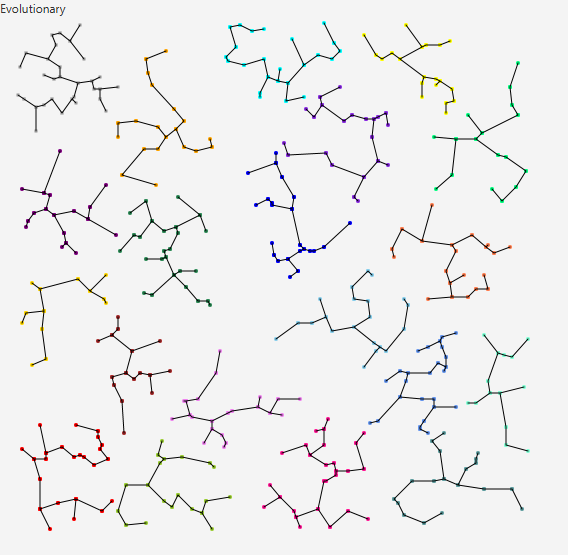
\includegraphics[width=0.45\textwidth]{sprawozdanie_6/evolutionary1.PNG}
        }
        \subfigure{
           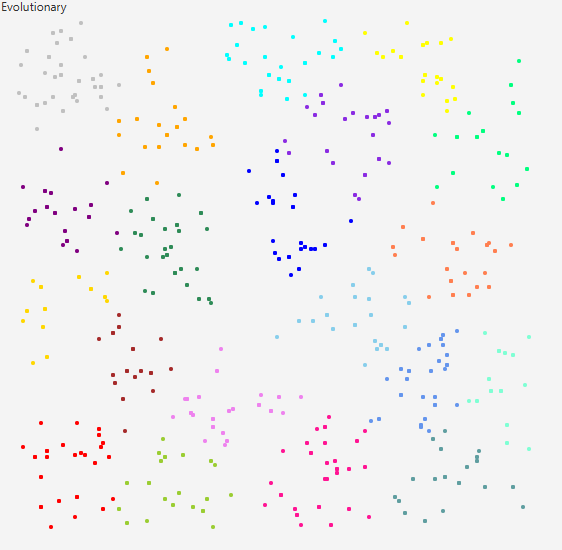
\includegraphics[width=0.45\textwidth]{sprawozdanie_6/evolutionary2.PNG}
        }\\
        \subfigure{
            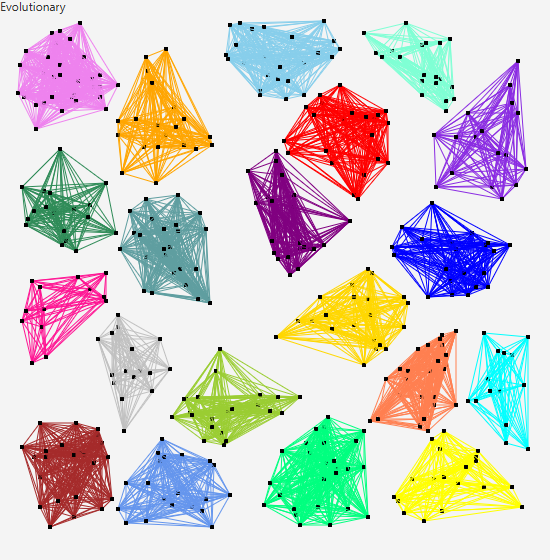
\includegraphics[width=0.45\textwidth]{sprawozdanie_6/evolutionary3.PNG}
        }
    \end{center}
\end{figure}


\end{document}